\documentclass[a4paper, twocolumn]{jarticle}
%\documentclass[uplatex]{jsarticle}
\usepackage[dvipdfmx]{graphicx}
\usepackage{float}
%\usepackage[dvips]{color}
%\usepackage{ascmac}
%\usepackage{verbatim}
\usepackage{setspace}
\usepackage[top=20mm,bottom=20mm,left=18mm,right=18mm]{geometry}
\makeatletter
\def\section{\@startsection{section}{1}{\z@}%
 {.1\Cvs \@plus.1\Cdp \@minus.1\Cdp}%
 {.1\Cvs \@plus.1\Cdp}%
 {\normalfont\normalsize\bfseries}}
\renewcommand{\thesection}{\arabic{section}.}
\renewcommand{\thesubsection}{\arabic{section}.\arabic{subsection}}
\def\subsection{\@startsection{subsection}{1}{\z@}%
 {.1\Cvs \@plus.1\Cdp \@minus.1\Cdp}%
 {.1\Cvs \@plus.1\Cdp}%
 {\normalfont\normalsize\bfseries}}

\def\@maketitle {
	\begin{center}
		\fontsize{14pt}{0pt}\selectfont
                % {\bf \@title{}}
                {\@title{}}
	\end{center}
	\vspace{1pt}
	\begin{flushleft}
		% \@author{指導教員 福田浩章 }
		\hfill{MA17099 古橋健斗}
	\end{flushleft}
\vspace{0.3cm}
}

%\makeatother
%\makeatletter

\renewcommand{\baselinestretch}{0.80}

\pagestyle{empty}
\makeatother

\begin{document}
\title{KAWAII Quest -ルンバの大冒険-}
\date{}
\maketitle
\thispagestyle{empty}

%%%%%%%%%%%%%%%%%%%%%%%%%%%%%%%%%%%%%%%%
%%背景と目的
%%%%%%%%%%%%%%%%%%%%%%%%%%%%%%%%%%%%%%%%
\section{研究の背景と目的}
はじめに,本研究で使用するロボットであるルンバと使用する技術である機械学習,使用するシステムである分散システムについて述べ,最後に本研究の目的を述べる.

\subsection{ルンバ}
ロボット技術の進化を背景に,近年様々な分野でロボットが活躍している.
中でも,掃除ロボットとして家庭で使用されているルンバ(図\ref{fig:roomba})\cite{irobot}は様々な研究で使われている\cite{thesis1}\cite{thesis2}.
ルンバはiRobot社が製造・販売するロボット掃除機である.
様々な型が存在するが,ルンバは直径34cmの円盤状で,高さは9cm以内,前方には接触センサーが組み込まれたバンパーがあり,上面の前方中央に赤外線センサーが搭載されている.
ルンバは掃除する部屋の地図を作成せずに,「らせん状に掃除する」「壁伝いに掃除する」「何かにぶつかったら角度を変えてランダムウォークする」などの単純なヒューリスティックスで動作している.
したがって,特定の箇所を何度も重複して掃除を行うことや一回,あるいは一度も通らないということも起きてしまうという欠点も存在する.

\subsection{機械学習を用いた画像認識}
機械学習を用いた画像認識は広く使われている.
機械学習とは,データから反復的に学習し,そこに潜むパターンを見つけ出すことである.
人手によるプログラミングで実装していたアルゴリズムを,大量のデータから自動的に構築可能になるため,さまざまな分野で応用されている.
機械学習のアルゴリズムには教師あり学習,教師なし学習,強化学習などがある.
教師あり学習は,入力とそれに対応すべき出力(ラベル)を写像する関数を生成する.
教師なし学習は,入力のみからモデルを構築する.
強化学習は,周囲の環境を観測することでどう行動すべきかを学習する.
行動によって必ず環境に影響を及ぼし,環境から報酬という形でフィードバックを得ることで学習アルゴリズムの指針とする.
これらのアルゴリズムから最適なものを見つけ,それを状況に応じて使用することでより精度の高い情報を得ることができる.

\subsection{分散システム}
近年サービスの効率化を目的として,単一のコンピュータで処理を行う集中システムから多数のコンピュータで処理を行う分散システムに移行している.
分散システムの利点として,複数のコンピュータで並列処理を行うので,処理が早い,拡張やスケールスケールが容易である,いつでも利用可能であるといったものがある.
大規模な分散システムを構築するには,システムの規模に応じたデータセンタが必要となる.
しかし,データセンタは高価なため,用意することがとても困難である.

\begin{figure}[tb]
	\centering
	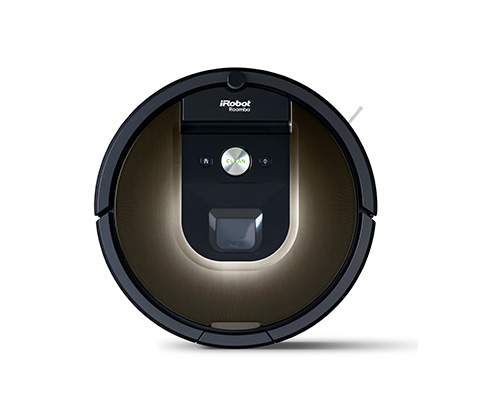
\includegraphics[width=8.0cm]{figure/roomba.jpg}
	\caption{ルンバ980}
	\label{fig:roomba}
\end{figure}

\section{本研究の提案}\label{subsec:a}
そこで,本研究では,ルンバを用いて対象物を発見し,機械学習を用いて対象物を判別し,データセンタを用いて分散的に処理を行うシステムを提案する.
データセンタが高価であるという問題は,小型計算機であるRaspberryPi(図\ref{fig:rpi2})を使用してデータセンタを模擬することで問題を解決する.
RaspberryPiは一台5千円弱であり,安価かつ省スペースでデータセンタの構成を模擬することができる.
実際にRaspberryPiを用いたデータセンタ環境構築の研究は行われている\cite{thesis3}.
また,今回の対象物の基準は可愛いものとする.
したがって,ルンバを徘徊させ対象物を発見し,可愛いものを判別し,それをRaspberryPiで構築されたデータセンタで分散的に処理することが本研究の目標となる.

ルンバには2つのモードを搭載する.
1つはユーザが自由にルンバを動かし,ユーザが可愛いと思う画像を撮影することで画像判別のための教師データの収集を行う.
これにより,感性の違いによる差異をなくす.
また,全ユーザに適用される教師データとそのユーザに対してのみ有効である教師データを分けることで,一定の教師データの確保をする.
もう1つは,ルンバが自動徘徊し,集めた教師データを元に可愛い対象物を発見,撮影し,ユーザへの表示を行う.
したがって,ルンバの操作や対象物の画像を表示するためにWeb上で使用できる管理ツールの作成を行い,ユーザは管理ツールを用いて本システムの管理を行う.

\begin{figure}[tb]
	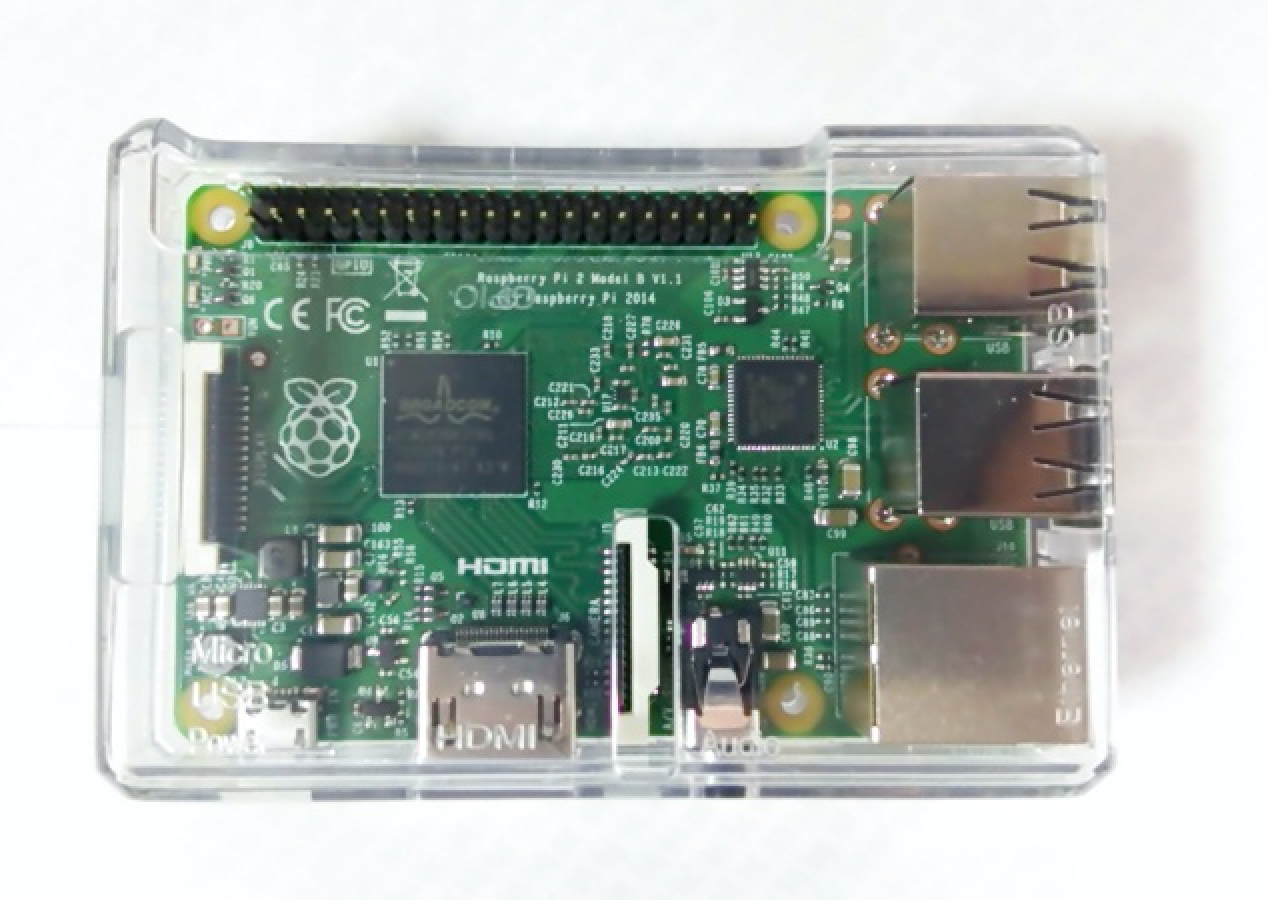
\includegraphics[width=8.0cm]{figure/rpi2.png}
	\caption{RaspberryPi}
	\label{fig:rpi2}
\end{figure}

%%%%%%%%%%%%%%%%%%%%%%%%%%%%%%%%%%%%%%%%
%% アプローチ
%%%%%%%%%%%%%%%%%%%%%%%%%%%%%%%%%%%%%%%%
\section{設計}
本研究では,RaspberryPiを用いた分散的に画像を処理を行うデータセンタ環境の構築と,ルンバの制御や状況管理を行う管理ツールの作成を行う.
データセンタ環境の構築には,動的なネットワークの構築と仮想マシンの起動・移動・複製が必要となる.
データセンタ環境の要件を以下に述べる.

\begin{figure}[tb]
	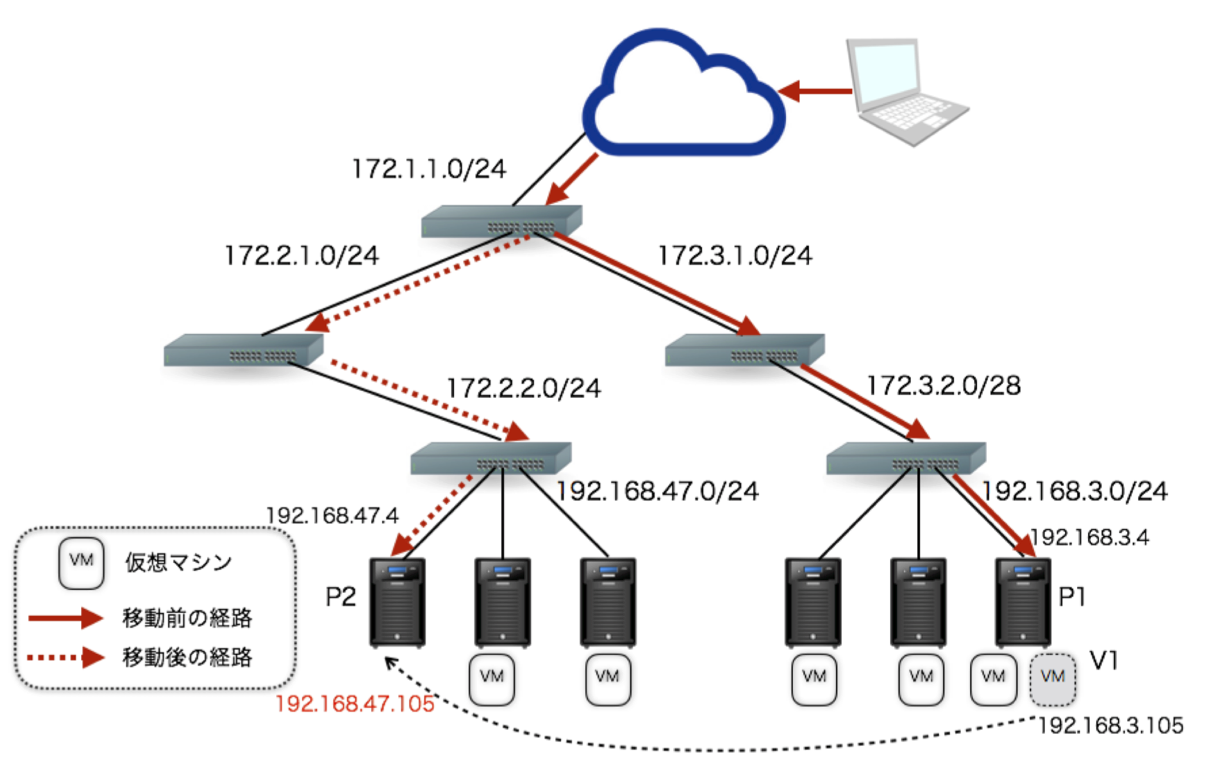
\includegraphics[width=8.0cm]{figure/cloud.png}
	\caption{想定するデータセンタ環境}
	\label{fig:cloud}
\end{figure}

\subsection{データセンタ環境}\label{subsec:cloud}
本研究で想定するデータセンタ環境を図\ref{fig:cloud}に示す.
データセンタ環境では,一般に複数のネットワークスイッチとそれらに接続した物理マシンで構成される.
ユーザからのリクエストはスイッチで適切に転送され,対象となる仮想マシンが適切に処理を行なっている.
ここで,物理マシンが高負荷になり,仮想マシンを移動する状況を想定する(図\ref{fig:cloud}).
図\ref{fig:cloud}では,物理マシンP1で仮想マシンV1が動作している状況において,V1を物理マシンP2に移動することを想定している.
P1とV1にはそれぞれIPアドレス(192.168.3.4, 192.168.3.105)が設定されており,ユーザの立場からは区別できない.
一方,P2にも192.168.47.4のIPアドレスが設定されている.
仮想マシンの移動では,一般にIPアドレスは変化しないため,V1のIPアドレスはP2に移動した後も変わらず192.168.3.105となる.
V1の移動はP2が直接接続しているネットワークスイッチ,および上流に位置するスイッチに影響しないため,従来V1に届けられていたパケットは依然として192.168.3.0/24を管理するスイッチに届けられることになり,移動後のV1に届けられることはない.
移動後のV1に正しくパケットを届けるためには,V1のIPアドレスと移動後のネットワークに合致したものに変更(e.g., 192.168.47.105)する必要がある.
加えて,ユーザからはこの変更は透過であるため,V1へのリクエストは依然として192.168.3.105宛に送信される.
したがって,ネットワークスイッチに変更を加え,宛先192.168.3.105へのパケットは変更後のアドレスに書き換えて(192.168.47.105)送信する必要がある.

このように,データセンタ環境で円滑に処理を行うためには,仮想マシンの移動や複製に伴い,関連するネットワークスイッチも連動して変更する必要がある.

\subsection{データセンタ環境の要件}\label{subsec:requirement}
\ref{subsec:cloud}節で述べたように,本研究で想定するデータセンタ環境の実現には,仮想マシンの移動だけでなく,IPアドレスの変更など,移動に伴う変更や,移動の契機となる状況の把握などが行える必要がある.
本研究のデータセンタ環境を実現するため,以下の項目をデータセンタ環境の必要要件と考える.

\begin{description}
\item [負荷状況の把握]仮想マシンの移動や複製は,一般に高負荷状態にある物理マシンの負荷を分散し,仮想マシンで提供するサービスの性能維持や,低負荷状態の物理マシンに散財する仮想マシンを集約し,リソースの効率的な使用ののために行われる.
本環境でもこれらの負荷状態を測定するため,負荷状態の判定に一般的に用いられるCPUとメモリ使用率を使用する.
また,物理マシンの負荷分散を目的として仮想マシンを移動させる場合,移動先物理マシンを決定する必要があるが,ネットワークを利用したサービスに主に用いられる環境ではネットワーク使用量も移動先を決定する指標となり得る.
そこで本研究では,物理マシン単体のネットワーク使用量だけでなく,スイッチ単位でのネットワーク使用量を測定し,移動先決定の指標に用いる.

\item [IPアドレスとルーティング管理]仮想マシンが移動する時,移動先物理マシンが同一ネットワークに所属している場合にはIPアドレスの変更は必要ない.
しかし,\ref{subsec:cloud}節でも述べたように,異なるネットワークに所属する物理マシンに移動する場合には移動後にIPアドレスの変更が必要になる.
同一ネットワーク内だけの移動/複製は,データセンタ環境の効率的な運用の妨げになるため,本研究ではネットワーク間を跨いだ仮想マシンの移動/複製も想定する.
その場合,複数の物理/仮想マシンに同一のIPアドレスを指定することはできないため,仮想マシン移動時にはIPアドレスを開放し,移動後には未使用のIPアドレスを設定できる必要がある.
さらに,ネットワーク間を跨いだ仮想マシンの移動/複製には,\ref{subsec:cloud}節で述べたように,IPアドレスの変更に伴い,関連するネットワークスイッチを変更し,適切にユーザからのリクエストを転送する必要がある.
\end{description}

\begin{table}[tb]
	\centering
	\caption{RaspberryPi2 ModelBの性能}
	\label{tab:rpi2}
	{
		\small
		\begin{tabular}{|c|c|} \hline
		CPU & ARM Cortex-A7 クアッドコア 900MHz\\ \hline
		メモリ & 1GB\\ \hline
		ネットワーク & 10/100Mbpsイーサネット\\ \hline
		電源 & 900mA(4.5 \textasciitilde 5.5W)\\ \hline
		\end{tabular}
	}
\end{table}

\subsection{RaspberryPIでの仮想化環境}
本研究のデータセンタ環境では\ref{tab:rpi2}に示すRaspberryPI2 ModelBを使用する.
CPUであるARMCortex-A7は仮想化拡張機能を備えているため,Linuxカーネルが備えるハイパーバイザ,KVMを実行することができる.

一方,\ref{subsec:requirement}節でも述べたように,本テスト環境の実現には仮想マシンの移動/複製に同期したネットワークの変更が必要になる.
近年,仮想化技術の進歩に伴い,ネットワークを柔軟に制御するためにSoftwareDefined Network(SDN)\cite{sdn}が注目を集めており,利用されている.
そこで本研究でもSDNを利用してネットワークを制御する.
本研究ではSDNの一種であり,広く利用されているOpenFlow\cite{opf}を利用するため,OpenFlow対応のソフトウェアスイッチであるOpen vSwitch(OvS)をRaspberryPiにインストールして利用する.
そのため,本データセンタ環境はすべてRaspberryPiだけで構成できる.

\subsection{負荷状況の把握}
負荷状況の指標として,各物理マシンのCPU使用率とメモリ使用率,各スイッチのトラフィック量を取得する.
物理マシンのCPUおよびメモリ使用量は物理マシンの/procディレクトリに格納されているファイルからリソース使用量を計算するプログラムを実装し,一定間隔(デフォルトは10秒毎)で実行してその値をデータベースに格納する.
また,トラフィック量の取得には,各OvSが計測している統計情報を元に各OvS全体,ポート毎のトラフィック量をそれぞれ取得する.
そして,これらの情報をOpen Flow ControllerであるOFCに送信し,OFCのデータベースに格納する.

\subsection{IPアドレスとルーティング管理}
本環境では,使用中のIPアドレスをデータベースで管理し,仮想マシンの起動や複製,移動時に次の手順で決定し,実際に設定する.
まず,移動先物理マシンが所属するネットワークアドレスを調べ,使用中のIPアドレス一覧を取得する.
次に,ネットワークアドレス,ブロードキャストアドレス,使用中のIPアドレスを除きランダムで決定する.
最後に,起動,複製,移動後の仮想マシンのifconfig,routeコマンドを使用してIPアドレスとデフォルトルートを設定する.

次に,異なるネットワークに仮想マシンの移動や複製を行う場合,OpenFlowを利用し,経由するOvSの設定を変更することで,パケットの転送経路を変更する.
具体的には,仮想マシンを移動する時,OFCはすべてのOvSのルーティング情報を保持ししているため,移動前アドレスのルーティングテーブルが存在するOvSを探索し,パケットを転送するポートを変更すると同時にパケットの送信先アドレスを変更する.
そして,移動後の仮想マシンから戻るパケットに関しては,送信元アドレスを移動前のアドレスに書き換えて送信する.
また,仮想マシンを複製する時には,移動と同様の処理を1/2の割合で実行することにより,ラウンドロビンで負荷を分散する.

\subsection{本データセンタ環境の分散システムの要件}
本研究で使用するデータセンタ環境は以下のような分散システムの要件を満たしている.

\subsubsection{透過性}
本環境では,アクセス透過性,位置透過性,移動透過性,複製透過性,並行透過性,障害透過性を満たしている.
\begin{description}
\item [アクセス透過性]
データセンタ環境に送られてきた画像は,仮想マシンで処理が行われる.
この仮想マシンを実行することができれば,いかなる物理マシンでもOSの差異を隠蔽することが可能である.

\item [位置透過性]
本環境ではOpenFlowによるパケットの振り分けを行うため,ルンバが転送する画像データの転送先は1つ知っていればよい.
例えば,データセンタ環境で仮想マシンV1と仮想マシンV2が起動しているとする.
その時,ルンバがV1のIPアドレスを知っていれば,OpenFlowが負荷状況により転送先を振り分けるので,V2のIPアドレスを知る必要がない.

\item [移動透過性]
本環境では仮想マシンの起動,複製,移動が行なわれるが,OpenFlowがパケットを書き換え,データの転送を行うので,ルンバは仮想マシンの状況を知る必要がない.

\item [複製透過性]
仮想マシンが(データごと)複製されるが,ルンバはそのことを考慮する必要がない.

\item [並行透過性]
共有リソース(機械学習の教師データなど)を複数の仮想マシンやユーザ間で共有することが可能である.

\item [障害透過性]
(仮想マシンを起動する)物理マシンに障害があっても問題なく動作する.
しかし,スイッチに障害があればその下にある物理マシンは使用不可能になる.
\end{description}

\subsubsection{スケーラビリティ}
・システムのサイズ
\begin{description}
\item [サービス]
データセンタ上では複数仮想マシンが起動しているので,ユーザが増えても問題なく処理が行われる.

\item[データ]
データセンタに新たに物理マシンを接続することでリソースを増やすことが可能である.

\item[アルゴリズム]
スイッチ上で負荷状況に応じて負荷分散を行うことでネットワークの負担を減らしつつ分散が可能である.
\end{description}

・分散型アルゴリズム

OpenFlowコントローラが全体ネットワークの情報(転送パケット数など)を管理しているが,局所的な情報しか持っていない.
また,仮想マシンは互いの情報を持っていない.
しかし,参照することは可能である.

・地理的な規模

物理マシンをデータセンタに繋げることで理論的に何台でも増やすことができ,それに応じてリソースを増やすことができる.

\subsection{管理ツール}
最後に,ユーザが本システムを使用するための管理ツールを作成する.
管理ツールに必要な要件は以下の通りである.

\subsubsection{管理ツールの要件}\label{tool}
はじめに,ユーザのログインが必要である.
なぜなら,ユーザ毎に画像認識を行うための教師データの選択が必要だからである.
そして,管理画面では,対象物の画像の表示と,ルンバの制御を行う.
ルンバには2つのモードがあることを\ref{subsec:a}節で説明した.
ルンバを制御するモードでは,管理ツールを通してルンバの移動や画像の撮影を行う.
自動徘徊モードでは,対象物の表示を行う.
また,どのルンバを制御するかを指定することも必要である.

%%%%%%%%%%%%%%%%%%%%%%%%%%%%%%%%%%%%%%%%
%%  実装・評価
%%%%%%%%%%%%%%%%%%%%%%%%%%%%%%%%%%%%%%%%
\section{実装・評価}
機械学習用のデータを処理するためのデータセンタ環境とユーザが本システムを使用するための管理ツールの実装を行う.

%%%%%%%%%%%%%%%%%%%%%%%%%%%%%%%%%%%%%%%%
%% 実装
%%%%%%%%%%%%%%%%%%%%%%%%%%%%%%%%%%%%%%%%
\subsection{実装}
\subsubsection{データセンタ}
本研究のデータセンタの構築風景を図\ref{fig:experiment}に示す.
このように,RaspberryPiを繋げ,内部で仮想マシンを複数起動する.
機械学習に用いる教師データや各教師データや物理マシンのリソース量はネットワークファイル共有システムであるNFSを用いて各物理マシンで同期が行われる.

\begin{figure}[tb]
	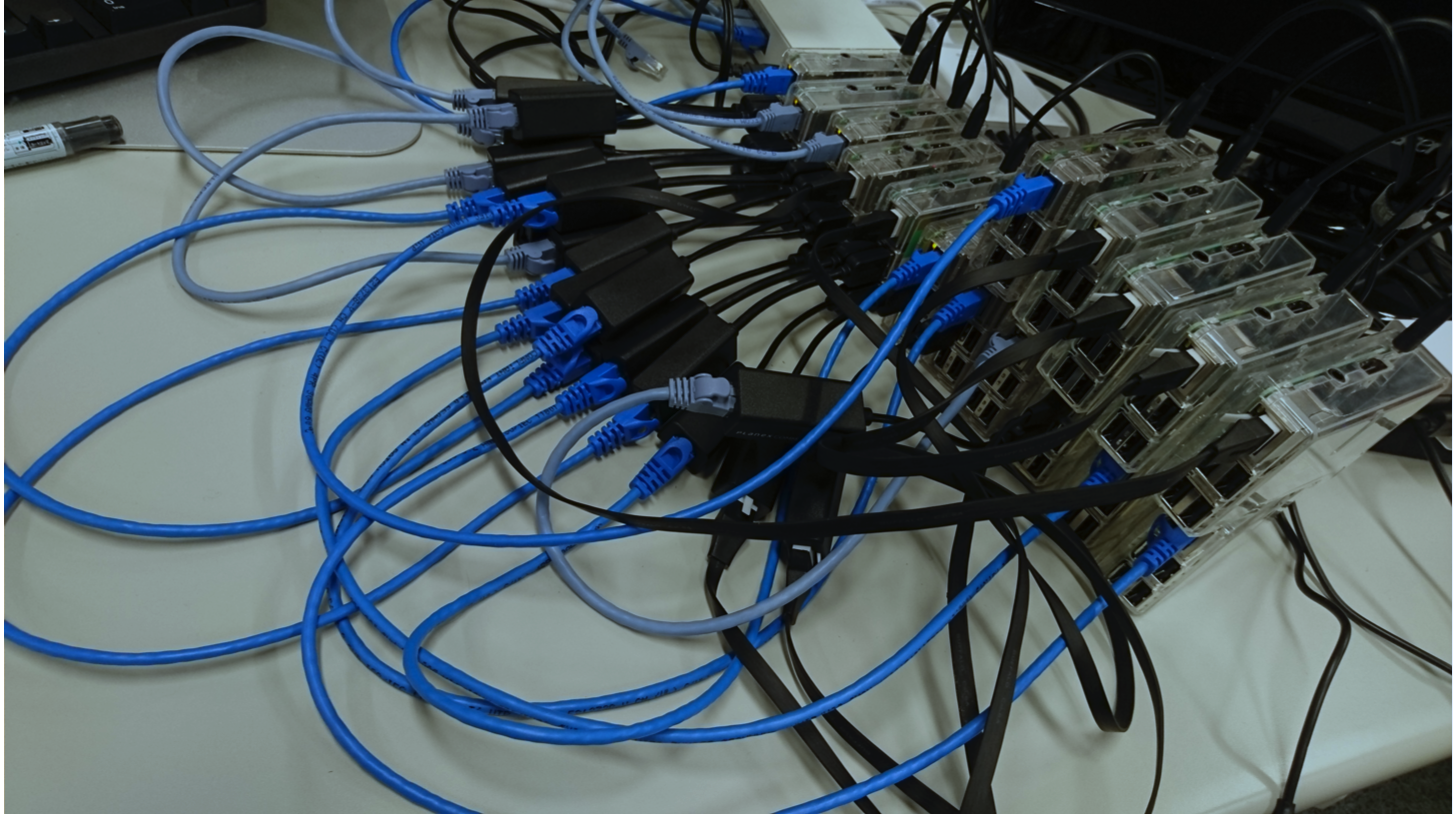
\includegraphics[width=8.0cm]{figure/experiment.png}
	\caption{RaspberryPiによるデータセンタ環境}
	\label{fig:experiment}
\end{figure}

\subsubsection{管理ツール}
\ref{tool}節で述べた通り,ユーザのログイン画面,管理画面を作成する.
設計はまだ行なっていない.
現在はルンバから送られてくる画像を動画のように表示する機能のみ実装を行なった.

%%%%%%%%%%%%%%%%%%%%%%%%%%%%%%%%%%%%%%%%
%% 関連研究
%%%%%%%%%%%%%%%%%%%%%%%%%%%%%%%%%%%%%%%%
\section{関連研究}
本研究では,RaspberryPiを用いたデータセンタ環境の構築を行った.
それに伴い,関連研究について述べる.

\subsection{The Glasgow Raspberry Pi Cloud:A Scale Model for Cloud Computing Infrastructures\cite{thesis3}}
この研究では,RaspberryPiを用いて教育用のデータセンタの構築を行なっている.
データセンタは高価で一般の学生などが触れることは少ないため,そのような人がデータセンタを使うための研究である.
しかし,この研究でのデータセンタは一般的なものであり,本研究では使用することができない.
なぜなら,この研究のデータセンタは負荷分散を行えず,画像処理などの負荷のかかる処理に対処できないためである.
本研究では,ユーザ毎に仮想マシンを指定するのではなく,負荷状況によって仮想マシンを指定する.
仮に,1つのルンバが大量の画像データを送った場合に,この研究のデータセンタでは全てのデータが1つの仮想マシンで処理が行われてしまうため,1つの仮想マシンに膨大な負荷がかかってしまう.
しかし,本研究のデータセンタは負荷状況に応じて画像データを振り分けるので,1つの仮想マシンに処理が集中することはなく,データセンタ全体で負荷の調整が行われる.
したがって,本研究のデータセンタは本システムにとって適したデータセンタ環境となっている.

%
% \subsection{SnowFlock\cite{thesis4}}
%
% \subsection{Reactive Cloud: Consolidating Virtual Machines with Postcopy Live Migration\cite{thesis5}}

%%%%%%%%%%%%%%%%%%%%%%%%%%%%%%%%%%%%%%%%
%% 今後の予定
%%%%%%%%%%%%%%%%%%%%%%%%%%%%%%%%%%%%%%%%
\section{今後の計画}
\begin{description}
    \item[データセンタの調節]

    ・本環境に合わせた負荷分散システムの構築

    ・教師データの作成を仮想マシン上で行うための設定

    ・必要ファイルの共有方法(おそらくNFS)の仕様

    \item[管理ツールの作成]

    ・本ツールからのルンバの操作

    ・ログイン画面(登録画面)

    ・ユーザデータベースの設計

\end{description}

%%%%%%%%%%%%%%%%%%%%%%%%%%%%%%%%%%%%%%%%
%%参考文献
%%%%%%%%%%%%%%%%%%%%%%%%%%%%%%%%%%%%%%%%
\begin{thebibliography}{9}
	{\small
    \bibitem{irobot}
    アイロボット公式サイト https://www.irobot-jp.com/roomba 2017-06-17

    \bibitem{thesis1}
    中村 彰宏, 大林 千尋, 柴田 智広, "ダンシングルンバ~踊る掃除制御~
Dancing Roomba", 情報処理学会研究報告 IPSJ SIG Technical Report 研究報告エンタテインメントコンピューティング(EC), Vol.2011-EC-20 No.10, 2011

    \bibitem{thesis2}
    福田 拓人, 森田 峰史, 高橋 智一, 鈴木 昌人, 青柳 誠司, "ロボット掃除機ルンバによる蛍光灯位置情報を利用した地図作成と自己位置推定(移動ロボットの自己位置推定と地図構築)", 一般社団法人日本機械学会 ロボティクス・メカトロニクス講演会講演概要集 2014, 2014

    \bibitem{thesis3}
    Fung Po Tso, David R. White, Simon Jouet, Jeremy Singer, Dimitrios P. Pezaros, "The Glasgow Raspberry Pi Cloud:A Scale Model for Cloud Computing Infrastructures",  2013 IEEE 33rd International Conference on Distributed Computing Systems Workshops, 2013

    \bibitem{sdn}
    Open Netrowking Foundation website. https://www.opennetworking.org 2017-06-17

    \bibitem{opf}
      Open Netrowking Foundation OpenFlow website. https://www.opennetworking.org/sdn-resources/openflow 2017-06-17

    % \bibitem{thesis4}
 %  	Horacio Andrés Lagar-Cavilla,Joseph Andrew Whitney,Adin Matthew Scannell,Philip Patchin,Stephen M.Rumble,Eyal de Lara,Michael Brudno,Mahadev Satyanarayanan,"SnowFlock:rapid virtual machine cloning for cloud computing,In EuroSys'09 Proceedings of the 4th ACM European conference on Computer systems", pp.1-12, 2009.
    %
    % \bibitem{thesis5}
    % Takahiro Hirofuchi, Hidemoto Nakada, Satoshi Itoh, Satoshi Sekiguchi, "Reactive Cloud: Consolidating Virtual Machines with Postcopy Live Migration", IPSJ Transactions on Advanced Computing Systems, Vol.5 No.2 86–98 ,2012

}
\end{thebibliography}
\end{document}
